\chapter{Considerações Finais}


\section{Resultados Parciais}

Após o acompanhamento das métricas de código-fonte do projeto \textit{Apache Maven} do dia 07/09/2013 a 10/11/2013, obteve-se as Figura \ref{table} e a Figura \ref{chart}, resultantes da implementação de algumas consultas OLAP  \textit{ad hoc}.



\begin{figure}[ht!]
\centering
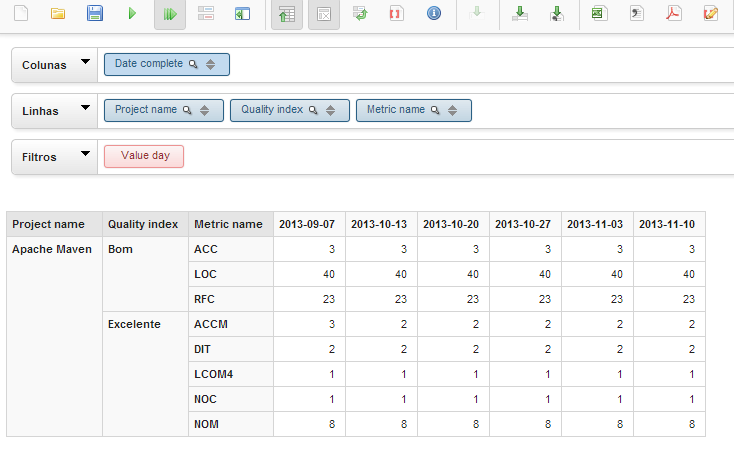
\includegraphics[bb=0 0 1257 350, scale=0.83]{figuras/indicadores.png}
\caption{Visualização de dados do Apache Maven em formato de tabela no Saiku Analytics}
\label{table}
\end{figure}
\FloatBarrier
 



\begin{figure}[ht!]
\centering
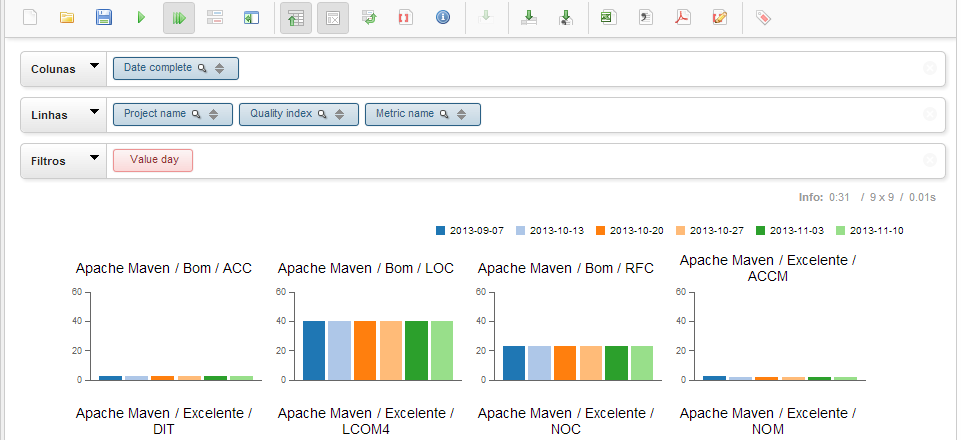
\includegraphics[bb=0 0 1257 350, scale=0.63]{figuras/indicadores_graficos.png}
\caption{Visualização de dados do Apache Maven em formato de gráfico de barras no Saiku Analytics}
\label{chart}
\end{figure}
\FloatBarrier

Após a implementação do ambiente de \textit{Data Warehousing} e a realização do estudo de caso sobre o ambiente,  verifica-se que a hipótese de pesquisa foi validada parcialmente. Isto é, o ambiente de DWIng possibilita maior poder de análise sobre as métricas de código-fonte. Isso ocorre porque a camada de visualização do ambiente de DWing permite uma flexibilidade de consultas que não está disponível nas ferramentas de análise estática de código-fonte e disponibiliza a informação da qualidade do código-fonte em formas visuais (gráficos e tabelas) as quais facilitam a interpretação da informação.


A análise dos gráficos e tabelas isolados na camada de visualização ainda não é a melhor forma de transmitir os dados, logo a hipótese deve ser verificada também quando for implementado o \textit{Dashboard}. 


Com a realização do estudo de caso da coleta de dados, das métricas de código-fonte do Apache Maven, observou-se que o comportamento de estabilidade das mesmas. Logo foi avaliado também a a média e mediana, como se mostra no apêndice \ref{metrics-data}.

Após a análise de média e mediana e percentis, corrobora-se com \citeonline{Meirelles2013}, pois a análise das métricas de código-fonte utilizando os percentis mostra valores representativos da qualidade geral do código-fonte. Mostra-se ainda, por meio da análise dos dados, que o Apache Maven é um projeto maduro e que, segundo os dados coletados, apresenta as métricas ACC, LOC, RFC em nível bom e as métricas ACCM, DIT, LCOM4, NOC, NOM em nível excelente.  



\section{Trabalhos Futuros}

Na próxima etapa deste trabalho, será \begin{inparaenum}[i)] \item melhor identificado outras demandas do negócio por meio de entrevistas semi-estruturadas com profissionais atuantes em métricas de código-fonte \item investigado a utilização de pesos para cada métrica de código-fonte, possibilitando assim configurações diferenciadas para cada projeto; \item avaliado as principais necessidades de informação em métricas de código-fonte, com objetivo de implementar o \textit{Dashboard} como componente de visualização; \item comparado o Pentaho com o SpargoBI, que também é uma outra ferramenta livre que possibilita o desenvolvimento do ambiente de DWing; \item implementado um estudo de caso em múltiplos projetos do ambiente de DWing. 
\end{inparaenum}
Com objetivo de distribuir as atividades de pesquisa e implementação, foi elaborado um calendário de marcos, tal como se vê na Figura \ref{calendar}.

\begin{figure}[ht!]
\centering
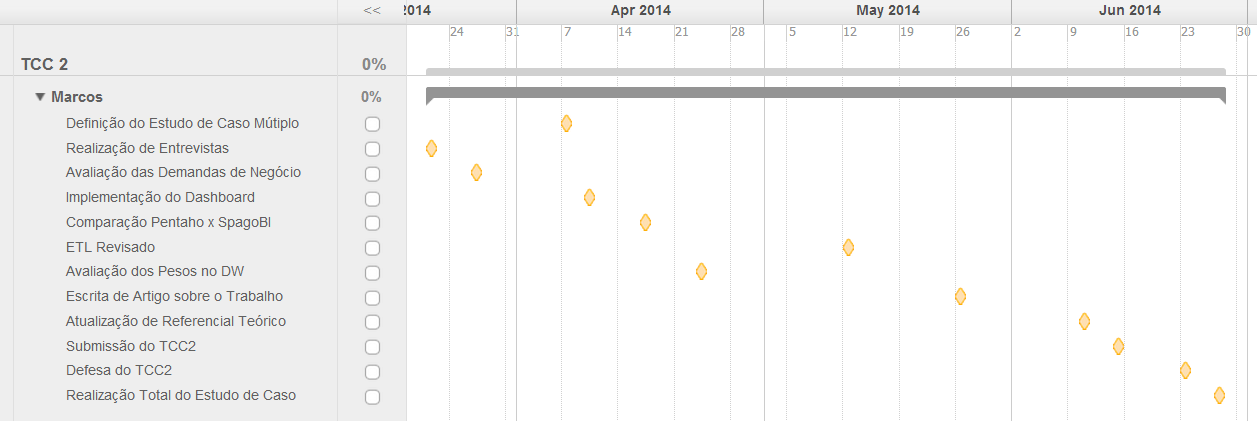
\includegraphics[bb=0 0 1257 350, scale=0.48]{figuras/tcc2-marcos.png}
\caption{Calendário de Marcos da próxima etapa deste Trabalho de Conclusão de Curso}
\label{calendar}
\end{figure}
\FloatBarrier
